\documentclass[final,hyperref={pdfpagelabels=false}]{beamer}
\mode<presentation>
  {
  \usetheme{ntnuposter}
  }

\usepackage{amsmath,amsthm, amssymb, latexsym}
\boldmath
\usepackage[english]{babel}
\usepackage[latin1]{inputenc}
\usepackage[orientation=portrait,size=a0,scale=1.7,debug]{beamerposter}
\usepackage{textcomp}
\usepackage{ragged2e}

\setlength\parskip{1.5\baselineskip}

% Column support
\setlength{\columnsep}{8em}
\usepackage{multicol}

% Scale down from a0 to a4
\usepackage{pgfpages}
\pgfpagesuselayout{resize to}[a4paper]


\title[NTNU-poster]{EIT-project -Group FUTHARK}
\author[Ervik et al.]{\AA smund Ervik, Paul Vo, Knut Halvor Skrede, Joakim Johnsen and Turid S. Solberg}
\institute[mia, NTNU]{MiA: Mathematics in Applications, Experts in Teamwork (Spring 2011), NTNU}
\date{2010-04-28}


\begin{document}
  \begin{frame}
  \begin{columns}[t]
  \begin{column}{.97\textwidth}

	\justifying

    \begin{multicols}{2}
	{\Large Introduction}

	Numerical simulations and experiments with bacon preparation
	in a microwave oven were performed. The numerical simulations were
	performed using the Crank-Nicolson numerical scheme on various heat
	equations for the different media in bacon. 
\\
The discetizaion scheme used was thus
\\
\begin{eqnarray*}
u_m^{n+1}-\mu k(\frac{1}{h^2}\delta_x^2 u_m^{n+1}-\frac{1}{f^2}\delta_y^2 u_m^{n+1}-\frac{1}{g^2}\delta_z^2 u_m^{n+1}) \\
=u_m^n + \mu k(\frac{1}{h^2}\delta_x^2 u_m^n + \frac{1}{f^2}\delta_y^2 u_m^n +\frac{1}{g^2}\delta_z^2 u_m^n)
\label{crank}
\end{eqnarray*}
\\
with truncation error of order
\begin{eqnarray*}
\frac{\tau_m^ n}{k} = \mathcal{O} (k^2 + h^2 + g^2 + f^2)
\label{truncerror}
\end{eqnarray*}
\\
The truncation error $\frac{\tau_m^n}{k} \Rightarrow 0$ as $h,f,g,k \Rightarrow 0$, and the Crank-Nicolson method is consistent for the heat equation. By performing a von Neumann analysis of the numerical scheme, one can show that the method are unconditional stable, thus the scheme converges.
\\
As boundary condition we used a constant temperature of 20 \textdegree C, which represent the roomtemperature. A source term, $J^{MW}$, was also added to the heat equation, to represent the microwave effect.
\\
\begin{eqnarray*}
  J^{MW}(r) &=& 0.5 + 2.55008r - 0.588013r^2 + 0.032445r^3 \\
    && + 0.00124411r^4 - 9.73516\cdot 10^{-4}r^5
  \label{eq:effektfordeling}
\end{eqnarray*}
\\
The experiments were
	performed with regular and with thick bacon in an ordinary household
	microwave oven, for single slices, and preparation times in the range
	30-70 seconds. The results of the experiments are in good agreement both
	with expected behaviour and with the results of the numerical work.
	
\vspace{1.0\baselineskip}
{\Large Result}

A program was written in C++, implementing equations given in the previous
section. The program produced an animation of heat distribution in the bacon, 
yielding the following plot at $t = 50$s:
\begin{figure}[!h] 
  \begin{center}
    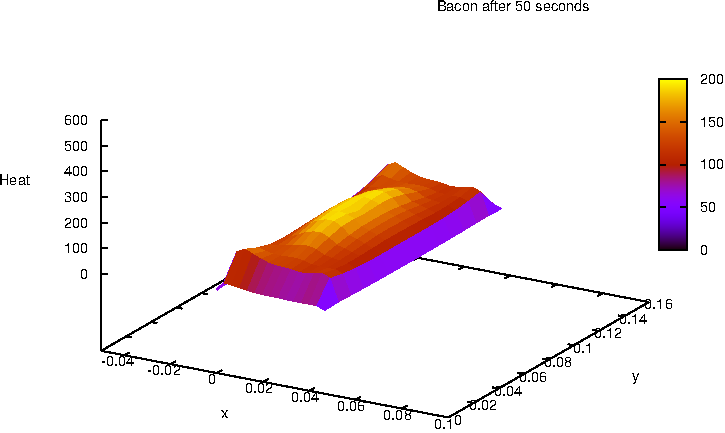
\includegraphics[width=\linewidth]{bacon-50sec.pdf}
  \end{center}
  \caption{A slice of bacon after fifty seconds in a microwave oven}
  \label{fig:bacon-50sec}
\end{figure}
By observing the plot in figure above we notice that the
temperature in the bacon slice is fairly close to $150^{\circ}$C. This is the required temperature
for initiation of Maillard reactions, thus the bacon is (according to theory)
cooked. This means that our numerical model predicts bacon completion at about
$50$ seconds, give or take.

    \vspace{1.0\baselineskip}	
The experiments yielded cooked bacon between $40-60$ seconds, depending on
desired degree of crispness. Bacon completion was predicted to coincide with a
critical temperature, as well as a limiting fat loss.
\begin{figure}[!h] 
  \begin{center}
    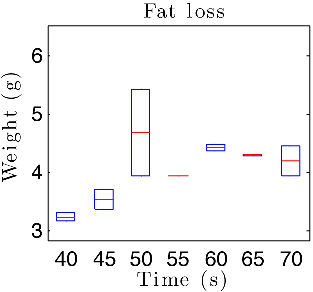
\includegraphics[width=\linewidth]{poster_bacon.pdf}
  \end{center}
  \caption{Experimental data regarding fat loss}
  \label{fig:bacon-50sec}
\end{figure}
As we can see in the figure above, there is clearly a limiting fat loss at about
$50$ seconds. This implies that our numerical model is accurate.
\vspace{1.0\baselineskip}
{\Large Conclusion}

    The performed numerical simulations and experiments with bacon preparation
in a microwave oven gave satisfactory results so far as they were implemented.
The numerical simulations of the heat equations gave reasonable results in agreement
with experiments. An implementation of the transport equation would have been
more satisfactory, and is suggested as a possibility for future work in this
direction. As microwave preparation of bacon is shown elsewhere to be the
healthiest option, expanding on the work here with more simulations and
experiments, and introducing a more complicated model of bacon fat at high
temperatures, one should be able to attain a complete understanding of the
preparation process and thus produce guidelines for the optimal preparation of
bacon.





    \end{multicols}



  \end{column}
  \end{columns}
  \end{frame}
\end{document}


%%%%%%%%%%%%%%%%%%%%%%%%%%%%%%%%%%%%%%%%%%%%%%%%%%%%%%%%%%%%%%%%%%%%%%%%%%%%%%%%%%%%%%%%%%%%%%%%%%%%
%%% Local Variables:
%%% mode: latex
%%% TeX-PDF-mode: t
%%% End:
